\section{LeNet-5}
LeNet-5 \cite{Lenet5} is the name of a cercain architecture of a convolutional network designed for handwritten and machine-printed character recognition. The net has been proved with MINST database, a database of handwritten digits that comes with the net.\\

%TODO ADD FIGURE OF THE ARCHITECTURE OF LENET

The basic architecture of Lenet is two convolutional layer, followed each one by a max pooling layer and then a fully-connected layer. This architecture could be visualized in figure X.

LeNet has been used to learn the implementation of convolutional neural networks, and LeNet is the basis of the network developed to carry out this project as it has been modified in order to adapt it to get this project goal. The code of LeNet-5 in Python could be found in \url{www.deeplearning.net}\\

The specifications of the downloaded LeNet code are the architecture of LeNet used for starting to work with this project is formed by two convolutional layers of size 5x5 and with 20 kernels in the first convolutional layer and 50 in the second one, those are followed (each one) by a max pooling-layer of size 2x2. Those four layer are followed by a fully-connected layer with 500 neurons at the output. The classifier which has been used is the logistic regression. The activation function of the convolutional layers and the logistic regression is tanh.\\

The learning rate is 0.1 and the network runs by 200 epoch. The data is split in thre sets: training, testing and validating. For each subset, when is fed to the network it is fed in batches, whose size is choosen by the user. Using batches is to prevent memory problems.\\

The training procedure is being realized for too many epochs as users has selected. While the trianing is being running, the validation is calculated for each epoch.

\url{www.deeplearning.net} is the original page of Theano where could be found tutorials, how to install and get it and the documentation of its functions.\\

\subsection{Structure of Lenet}
LeNet works basically with theano although it uses others libraries like NumPy.\\

First of all in Lenet the data is loaded. The function that download the data check, firstly, if the data is not downloaded yet, if it downloaded it does not repeat the download. The data is downloaded split into train, test and validation subsets.\\

After loading the data, the architecture is defined, the layers are called because they has been defined as objects, each kind of layer, one different object. There is a object for convolutional + maxpooling, another object for the hidden layers that is a fully connected layer, and the classifier used that is logistic regression. Each part of the code could be found in \url{www.deeplearning.net}\\

After creating the structure, the functions of training, validating and testing are created as Theano functions.\\

In a big while loop the training validation and testing is developed. The data is trained. Each mini-batch (that is a small quantity of that given by the user, it is used in order to not train or test all the data together because it would take too much computer resources) is trained and the weights and bias of each layer are updated. It is given a validation frequency, this parameters decides how many validations are produced. So the data is trained and validation, when a best score of validation is produced, the data is tested.\\

The training would run for a number of epoch that the user has given or by a early-Stopping that has been developed by authors. The early-stopping combats over-fitting by monitoring the model's performance on a validation set.\\

\subsection{Results of LeNet}
The result of the network using the given database could be seen in figure \ref{fig:Lenetresult}, where the least error in validation performance is 0.91 \% obtained at iteration 18300, with an error test performance of 0.92 \%. \\

\begin{figure}[htb]
\centering
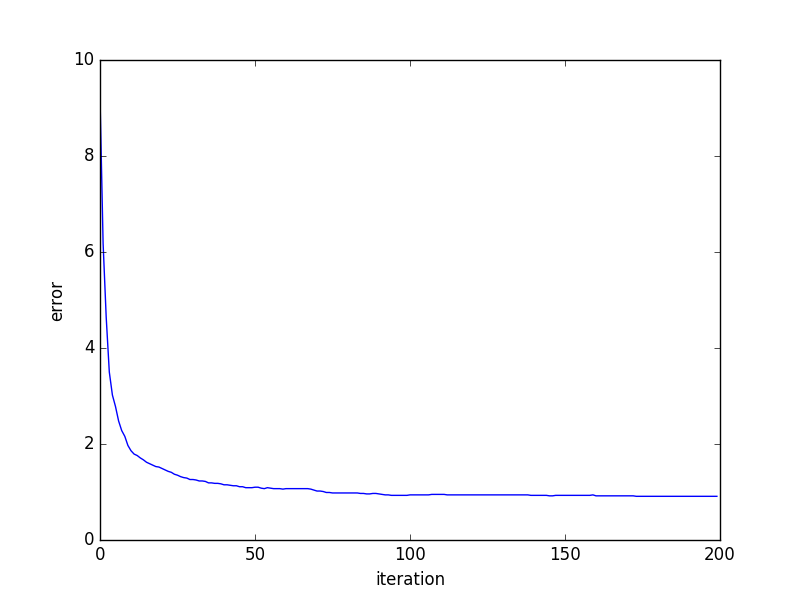
\includegraphics[width=0.7\textwidth]{images/ModificandoLenet/error_lenet.png}
\caption{Validation error obtained with Lenet and MNIST digits database} \label{fig:Lenetresult}
\end{figure}

It is important optimize the cost function, so it is possible to analyze how the networks works looking the cost function. The cost produced at the training gets reduced with the increasing iterations, as it is seen in figure \ref{fig:Lenetcost}.\\

\begin{figure}[htb]
\centering
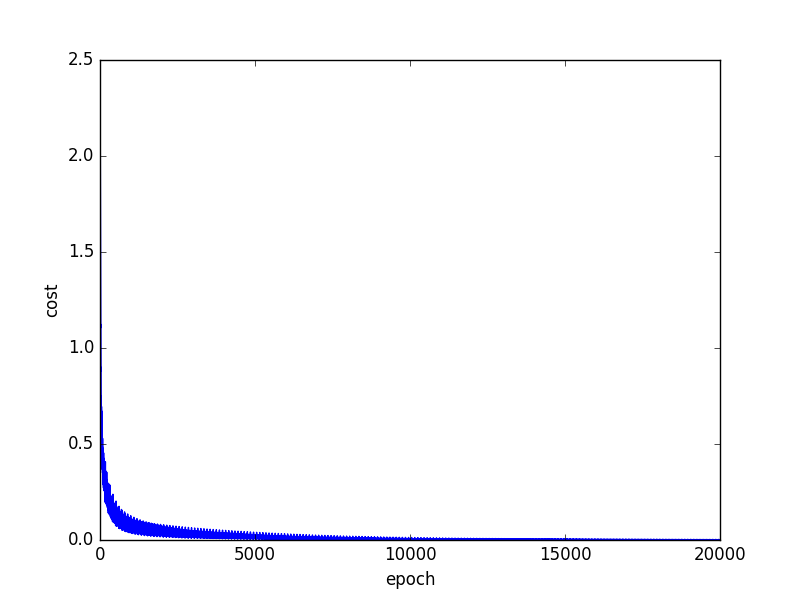
\includegraphics[width=0.7\textwidth]{images/images_lenet/cost_lenet.png}
\caption{Cost function of running Lenet with it is own database.} \label{fig:Lenetcost}
\end{figure}

As it is known, weights are filters, twenty first weights of each convolutional layers are shown in figure \ref{fig:weights_lenet} of the tenth and hundredth epoch.\\

\begin{figure}[htb]
\centering
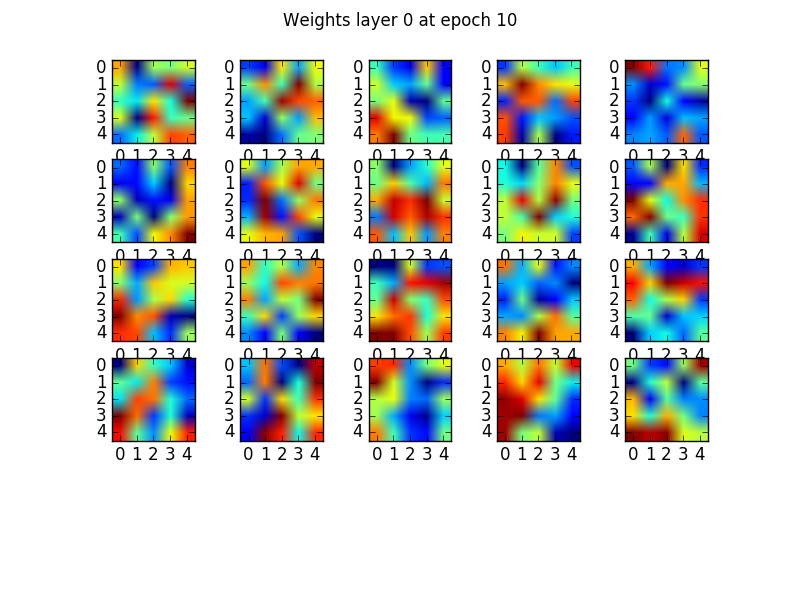
\includegraphics[width=0.48\textwidth]{images/images_lenet/w_layer0_epoch10.png}
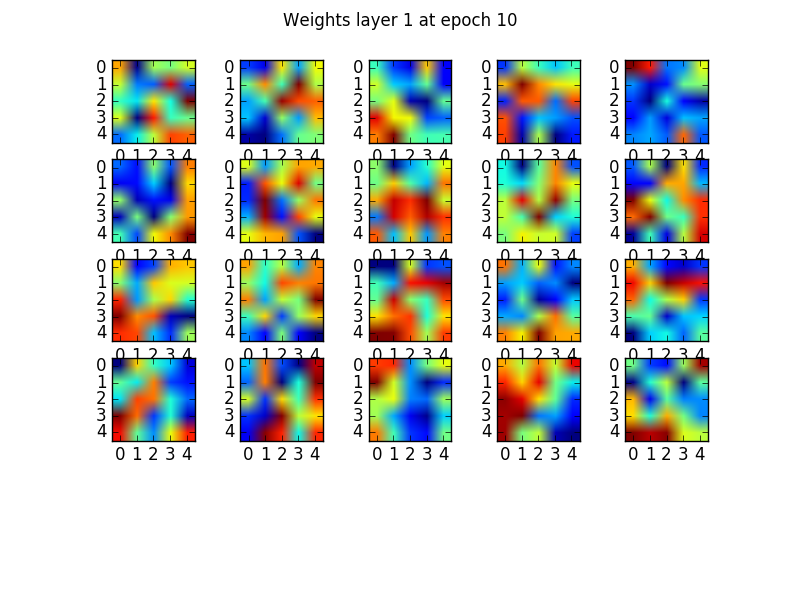
\includegraphics[width=0.48\textwidth]{images/images_lenet/w_layer1_epoch10.png}
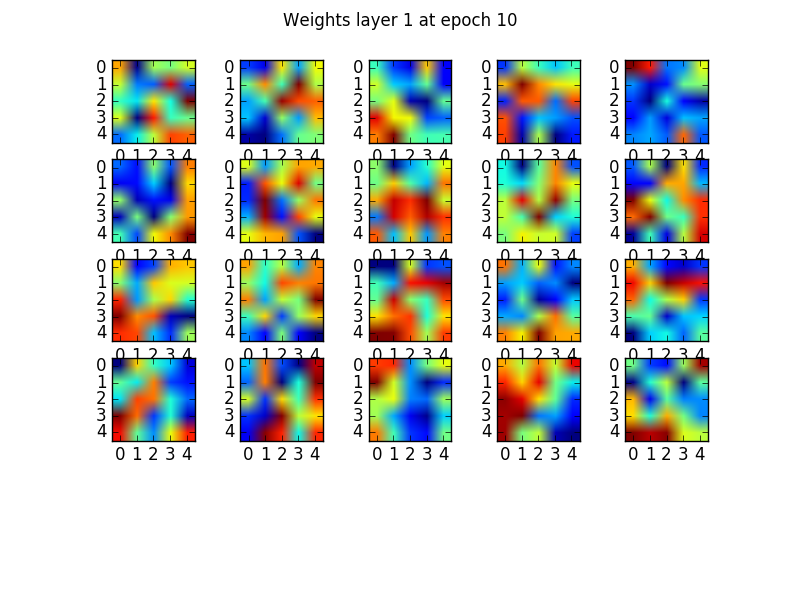
\includegraphics[width=0.48\textwidth]{images/images_lenet/w_layer1_epoch10.png}
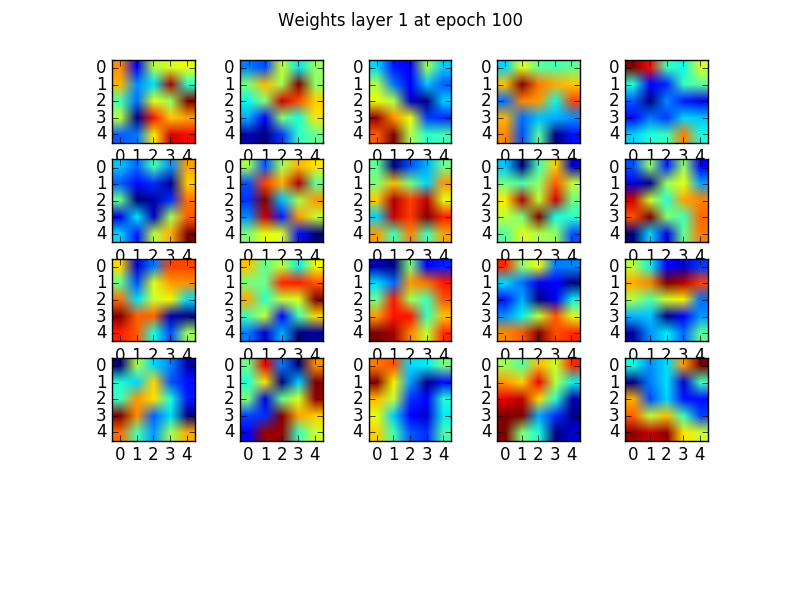
\includegraphics[width=0.48\textwidth]{images/images_lenet/w_layer1_epoch100.png}

\caption{Weights at epoch 10 and 100 of the two convolutional layers } \label{fig:weights_lenet}
\end{figure}

While the network is learning, weights change and they would not have the same apparence if were represented. \\


%The neural network has beoen built in Python using Theano library. The %network has been based on the one exposed in \textit{Learn Convolutional %Neural Network for Face Anti-Spoofing} and \textit{LeNet}.\\

%The architecture of the network is formed by two convolutional layers which %is followed (each one) by a max-pool layer.The  last max-pool layer is %followed by a fully-connected layer which have sigmoidal activation %function.\\

%The rectified linear activation function (reLu) is used as activation %function of the convolutional layers. It has been used a normalized %distribution of weights and bias, the same which was implemented in LeNet: %weights are sampled randomly from a uniform distribution in the range [-1/%fan-in, 1/fan-in], where fan-in is the number of inputs of the previous %layer. The ReLu function that has been used is the one implemented in %theano as theano.tensor.nnet.relu.\\

%The number of kernels used in the conv layers are 48 and 96 of size 5x5, %the size of the max-pool layer is 2x2.\\

%The network is trained with the 70\% of the data, the 30\% is used to test. %From the 70\% of the training data, the 25\% is used to validation.\\

Each time we take a sample and update our weights it is called a mini-batch. Each time we run through the entire database, it's called an epoch. Batch size determines how many examples you look at before making a weight update. The lower it is, the noisier the training signal is going to be, the higher it is, the longer it will take to compute the gradient for each step. \url{http://stats.stackexchange.com/questions/140811/how-large-should-the-batch-size-be-for-stochastic-gradient-descent}.\\


To be sure that the batch size do not affect to the results, it has been changed, in first place into 20 and in second place into 100. In the fist example (when batch size = 20), the while has been break because of early-stopped at epoch 31, from epoch 16 the networks does not improve the validation result.\\

In figure \ref{figures:LENET-batches} the error in each epoch is represented  for 500 batch size, the original size, for a value of 20 and 100. In the original case, the error stars with a value of 9\% aprox. with the batch size = 20 the error in the first iteration is about 2.4\%, and with a bunch of 100 images, the validation error is 3.5\%.

With the original size and size equal to 20, it is possible to get to the same minimum, the difference between those examples is that each one get to that conclusion into different epochs. With a batch size equal to 100, the code stopped because of the early-stop with a patience of 10000; it stop in epoch 33,while those epochs, it has been possible to get to a test error of 1.04\% in iteration 8500 when the validation error was 1.01\%, it has been running with put getting a better validation score for 17 epoch. With a batch size = 20, the code also has stopped earlier because of the same reason, but in that case it has been possible to get to the same minimum that with the original size; the epoch in which has stopped is 31, it has been running without getting a better validation score for 15 epochs.\\

\begin{figure}[htb]
    \centering
	\subfigure[batch size = 500 (original size)]{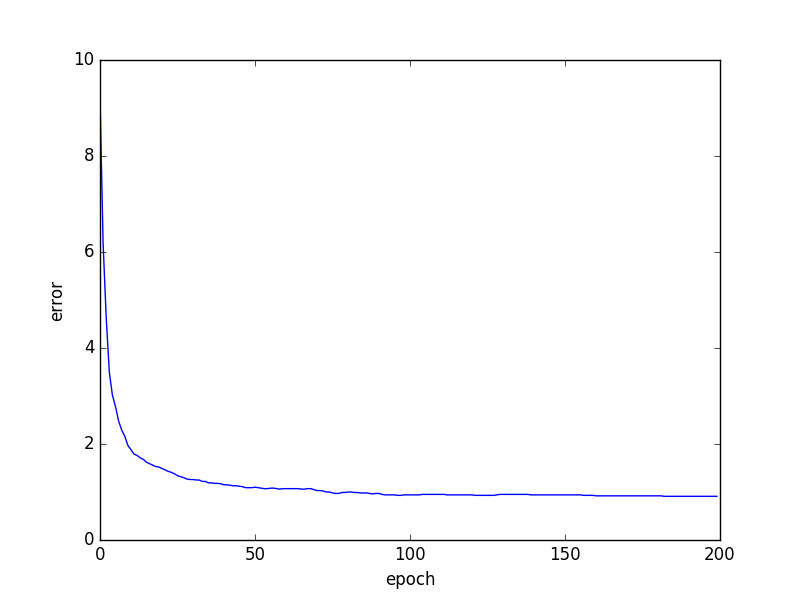
\includegraphics[width=0.47\textwidth]{images/images_lenet/lenet_batch/lenet_500batch_rror.png} }
	\subfigure[batch size = 20]{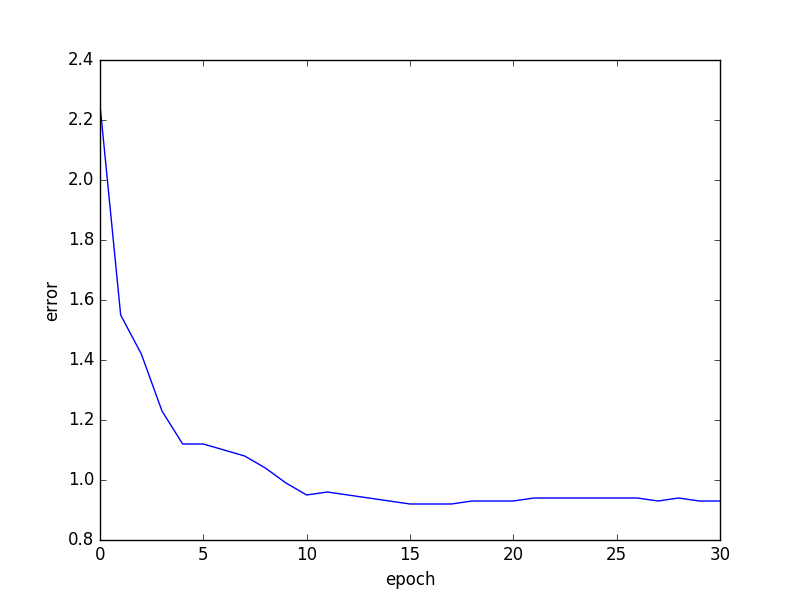
\includegraphics[width=0.47\textwidth]{images/images_lenet/lenet_batch/lenet_20batch_error.png} }
	\subfigure[batch size = 100]{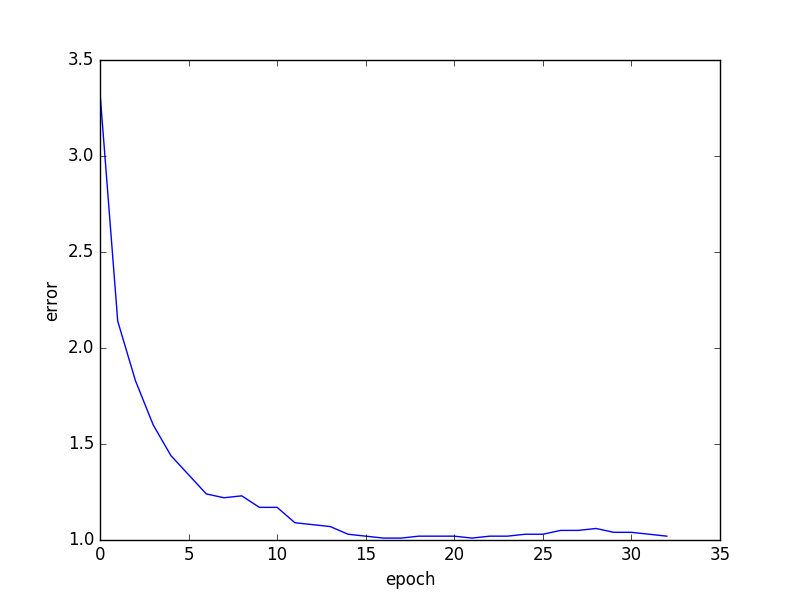
\includegraphics[width=0.47\textwidth]{images/images_lenet/lenet_batch/lenet_100batch_error.png} }

    \caption{Validation error in each epoch for diferentes sizes of batches.} \label{figures:LENET-batches}
\end{figure}

If the patience is increased from 10000 to 100000 for a batch size = 20 and equal to 100, results obtained are that for a value of 20, it has been running for 40 epoch, having the same results that the one obtained with a patience of 10000.\\

 For a value of 100 with the patience increased to 100000, the results are not the same as the one obtained the patience equal to 10000. In this occasion, the results are better than in the original one; The code has run for 258,08 minutes and for 200 epochs. The result obtained was better than in the original one has it has said. In epoch 51 has gotten a validation error of  1 \% and the error test has been 0,89\%, from this point, the test error that has been calculated five more times, has been increasing until get the value 0,85\% in iteration 55500, epoch number 111, the validation error obtained has been 0,95\%. From this epoch until number 200, the network has not had any better result.\\

In figure X it is possible to see the error function for those two examples. It could be seen that the example with batch size = 20 has just run for 40 epoch and the good results of the example with batch size = 100, remembering that the patience has been increased from 10000 to 100000.\\

\clearpage
\subsection{Modifying LeNet}
From LeNet, with the database gray scale digit database, the one that LeNet uses in the original example (grey scale images whose size is 28x28), some modification has been realized:\\

\begin{itemize}
\item{Using Local Response Normalization (LRN) In which a normalization has been carried out in the convolutional-max pooling layers.}
\item{Using ReLu as activation function:} The activation function tanh has been substituted by ReLu activation function in convolutional and fully connected layers.
\item{Using Relu and LRN}: The activation function used is ReLu and LRN has been used as  normalization layer.
\item{Change weights initialization}: Weights initialization has been changed by Gaussian. In which mean value that has been used is 0 and std is 0.01. Weights initialization has been changed in convolutional and fully connected layers. Also, bias initialization has been changed by ones.
\end{itemize}

%Using Local Response Normalization we want to detect high frequency features with a large response. If we normalize around the local neighborhood of the excited neuron, it becomes even more sensitive as compared to its neighbors.[\url{https://prateekvjoshi.com/2016/04/05/what-is-local-response-normalization-in-convolutional-neural-networks/}].\\

First, the cost of training process are going to be visualized with the original cost train, without modifying LeNet). In figure \ref{fig:CostModLeNet} is represented. Also the validation error (validation cost*100) could be visualized in figure \ref{fig:CostModLeNet}. The network has been running for 200 epochs.\\

\begin{figure}[htb]    \centering
	\subfigure[Original LeNet]{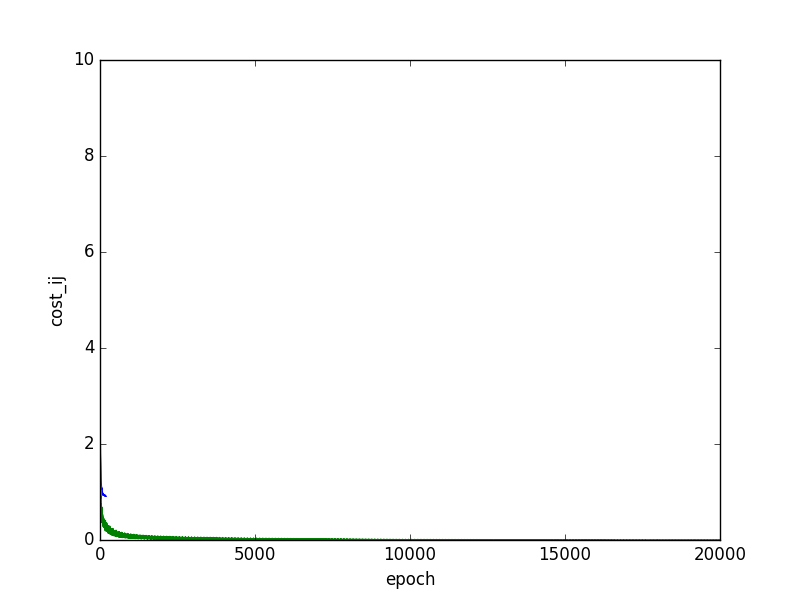
\includegraphics[width=0.42\textwidth]{images/ModificandoLenet/cost_lenet.png}\label{fig:cost_lenet} }
	\subfigure[Using LRN]{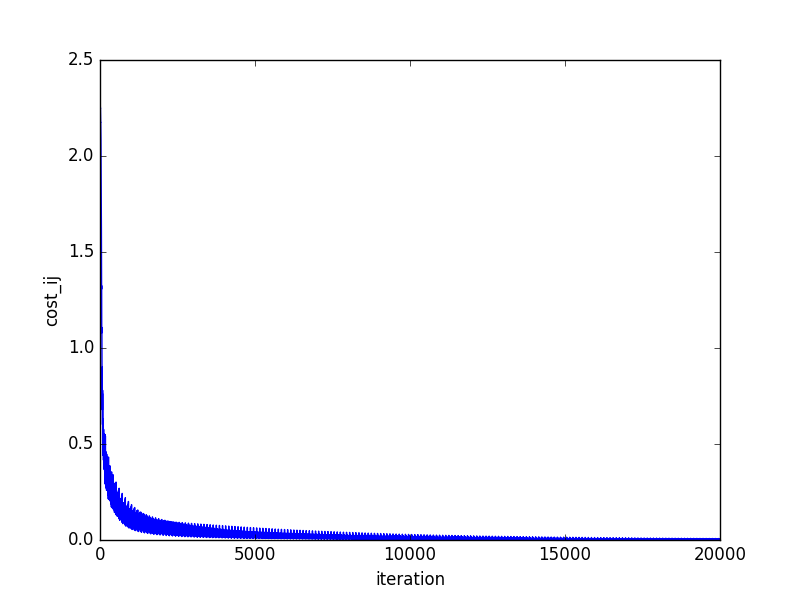
\includegraphics[width=0.42\textwidth]{images/ModificandoLenet/cost_lenet_LRN.png}}
	\subfigure[Using ReLu]{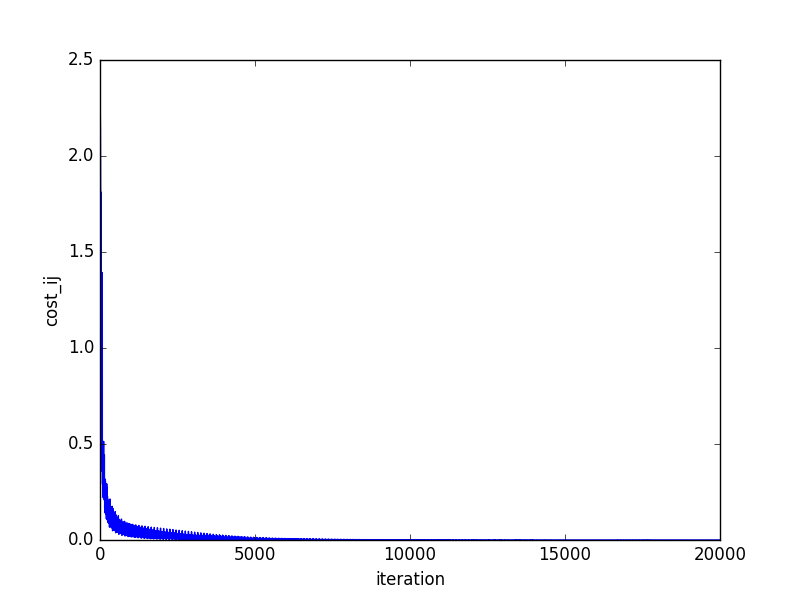
\includegraphics[width=0.42\textwidth]{images/ModificandoLenet/cost_lenet_relu.png}}
	\subfigure[Using ReLu and LRN]{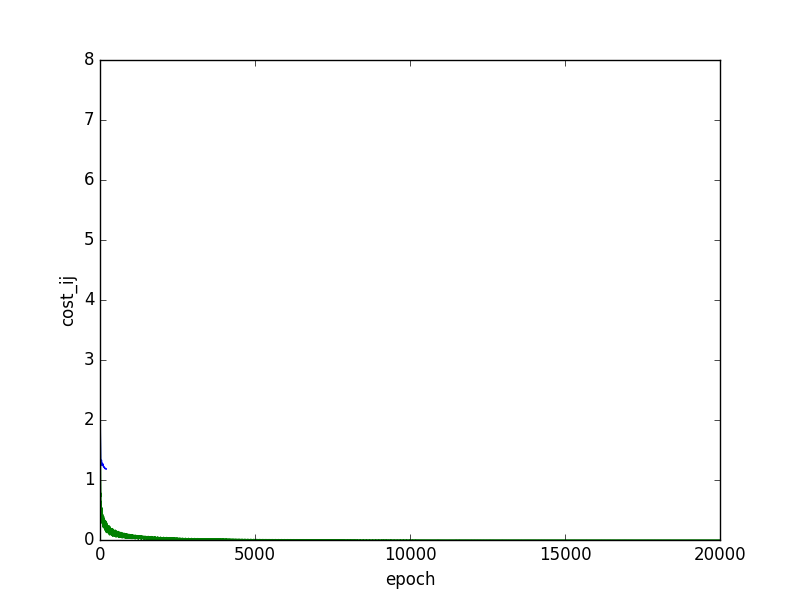
\includegraphics[width=0.42\textwidth]{images/ModificandoLenet/cost_lenet_relu_lrn.png}}
	\subfigure[Using Gaussian weights init.]{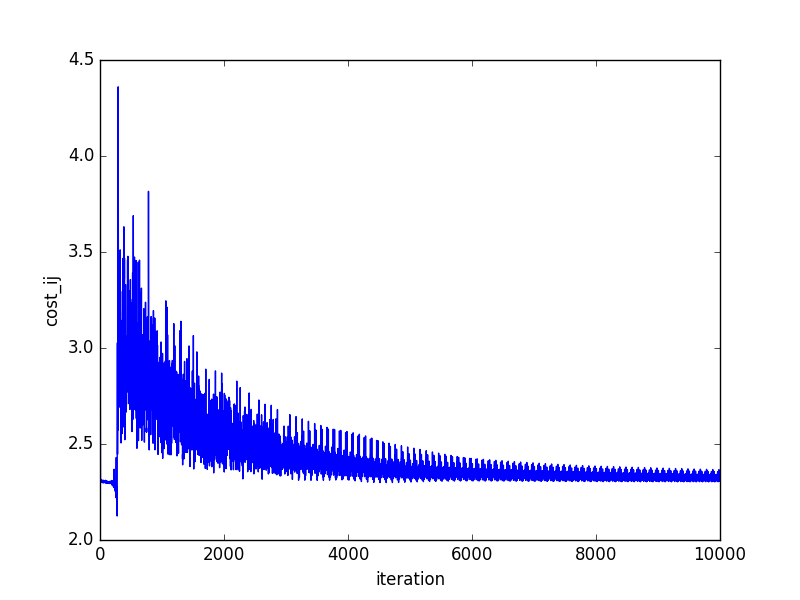
\includegraphics[width=0.42\textwidth]{images/ModificandoLenet/cost_lenet_gausianInit.png} \label{fig:cost_gaus_lenet}}
    \caption{Cost function of Lenet and Lenet Modified.} \label{fig:CostModLeNet}
\end{figure}

Visualizing the loss during the training, could be affirmed that the network with Gaussian initialization is in a local minimum because the loss has converged as could be seen in figure \ref{fig:cost_gaus_lenet}. The loss of LeNet without being modified (figure  \ref{fig:cost_lenet}) is the one whose oscillation at training is less than others.\\\\

\begin{figure}[htb]    \centering
	\subfigure[Original LeNet]{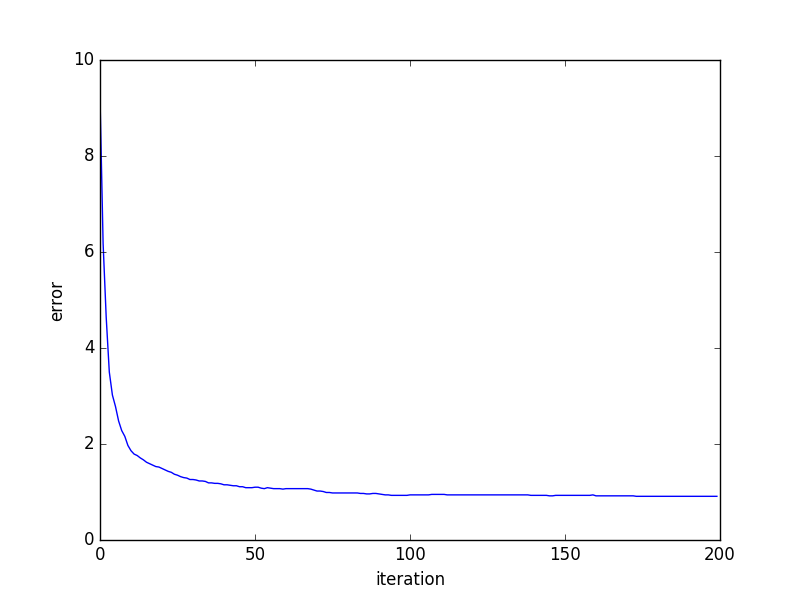
\includegraphics[width=0.42\textwidth]{images/ModificandoLenet/error_lenet.png}\label{fig:error_lenet} }
	\subfigure[Using LRN]{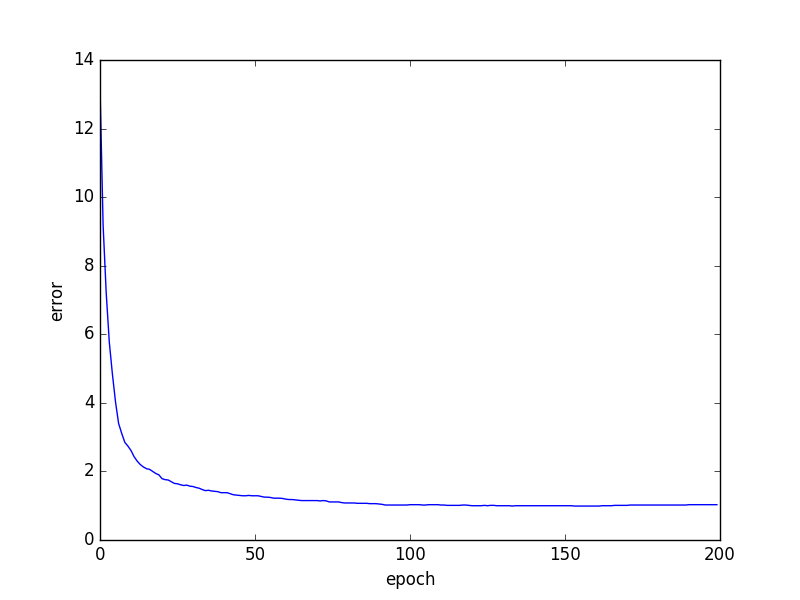
\includegraphics[width=0.42\textwidth]{images/ModificandoLenet/error_lenet_LRN.png}}
	\subfigure[Using ReLu]{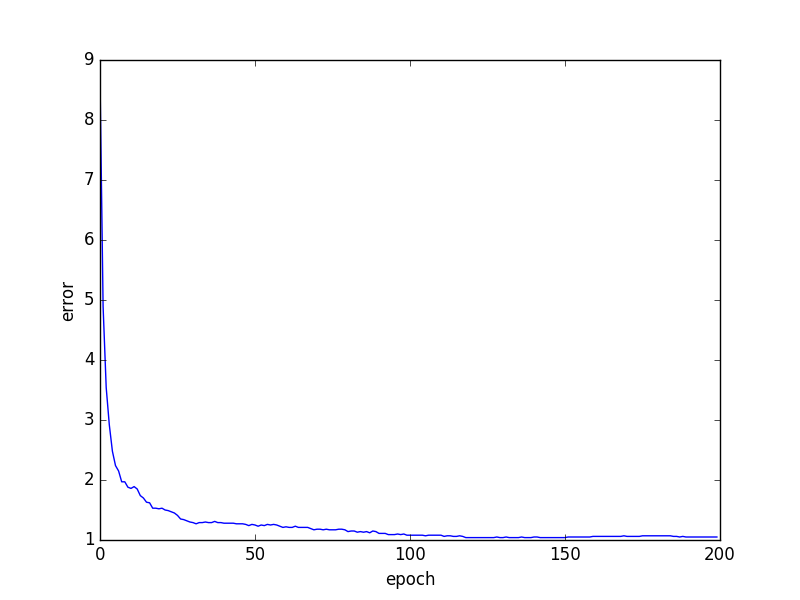
\includegraphics[width=0.42\textwidth]{images/ModificandoLenet/error_lenet_relu.png}}
	\subfigure[Using ReLu and LRN]{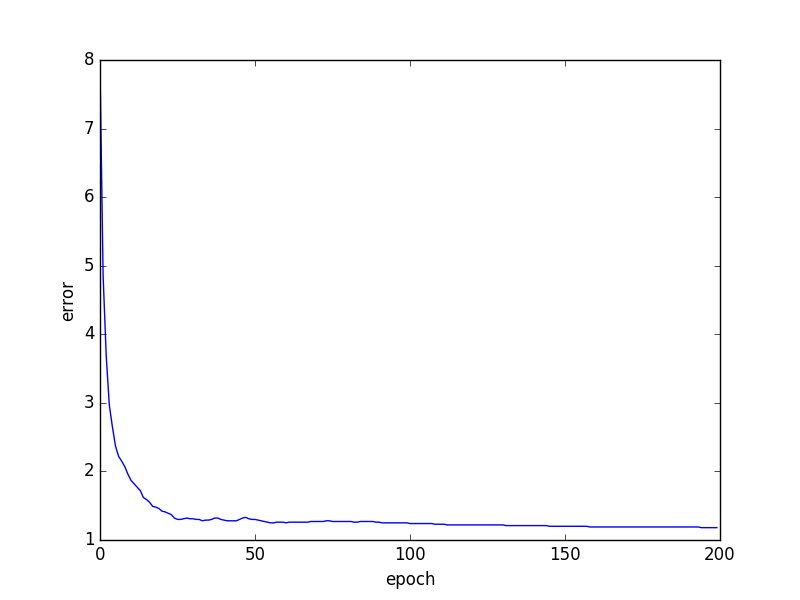
\includegraphics[width=0.42\textwidth]{images/ModificandoLenet/error_lenet_relu_lrn.png}}
	\subfigure[Using Gaussian weights init.]{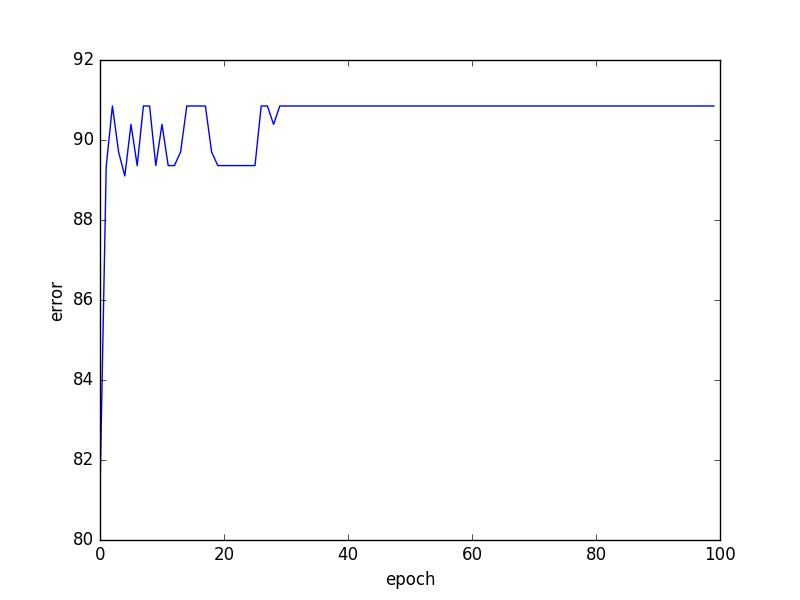
\includegraphics[width=0.42\textwidth]{images/ModificandoLenet/error_frav_gausianInit.png} \label{fig:error_gaus_lenet}}
    \caption{Valid error of Lenet and Lenet Modified.} \label{fig:ErrorModLeNet}
\end{figure}

About the error at validation, visualizing the graphs in figure \ref{fig:CostModLeNet}, it is very similar the curve for original lenet, lenet with ReLu, lenet with LRN and lenet with LRN and ReLu.

At testing, the results obtained have been the following ones:

\begin{itemize}
\item{Original LeNet}: Best validation score of 0.91 \% obtained at iteration 17400, with test performance 0.92\%.
\item{Using Local Response Normalization}: Best validation score of 0.99 \% obtained at iteration 13400, with test performance 1.6 \%.
\item{Using ReLu as activation function}:Best validation score of 1.04 \% obtained at iteration 11900, with test performance 2.4\%.
\item{Using Relu and LRN}: Best validation score of 1.18 \% obtained at iteration 19500, with test performance 1.08 \%.
\item{Gaussian weight initialization}: Best validation score of 81.22\% obtained at iteration 100, with test performance 80.90\%.
\end{itemize}

The best configuration for the network is the original one. With Gaussian initalization, the network does not find a local minimum in such a sort of time. Using LRN and Relu, test result is closer to the obtained with LeNet original, but not as good as the last one. Changing the activation function has not been a good change. Not taking into account original LeNet, the best test performance has been obtained with 1,08\% using ReLu and LRN, but the best validation error is 0,99\% obtained using just LRN. The values are close of the modifications, but the modification of Gaussian weight initialization.\\

\clearpage
